%%%%%%%%%%%%%%%%%%%%%%%%%%%%%%%%%%%%%%%%%%%%%%%%%%%%%%%%%%%%%%%%%%%%%%%%%%%%%%%%
\subsection{Wide-Area Performance and Fault Tolerance}
\label{cloud-measure-performance} 


Our results in the last section revealed that several services, even
highly ranked Alexa domains, appear to use only a single region or
even just a single availability zone.  In this section, we explore the
impact of these choices on web services' wide-area performance and
tolerance to failures.  We focus on EC2-using web services.


\subsubsection{Wide-area Performance} 


The choice of region(s) by a cloud service may impact performance in
at least two ways. First, clients' geo-distribution may
be poorly matched to particular regions; such clients may experience
poor latency and throughput compared to a more
judicious deployment. Second, there could be temporary changes in
which region performs best for a client due to 
congestion~\cite{akella2003empirical} or routing
problems~\cite{teixeira2004dynamics}.
%Deploying cloud services in multiple regions has the potential to help
%improve user experience here as well.

While the impact of diverse deployment of services (e.g., via CDNs)
has been previously studied in other
settings~\cite{krishnan2009moving}, we are unaware of any studies that
assess its impact for the available diversity of modern public IaaS
clouds. We therefore perform measurements to help us answer the
following two questions: ({\em i}) To what extent does the choice of region
impact performance experienced by clients of a web service? ({\em ii}) To
what extent does the use of multiple regions (or zones) improve the
client-perceived performance?


\tightparagraph{Latency measurements.}  To study per-region latency
performance, we set up 40 m1.medium instances, 2 in each of the 20
availability zones available to us on EC2. 
We selected 80 geographically distributed
PlanetLab~\cite{planetlab} nodes as stand-ins for real clients and we
used the hping3 utility to conduct 5 TCP pings to each of the 40
instances, from which we derive the average RTT. Pings that timed out
were excluded from the calculations of the average.
% The average RTT was computed as the average of these 5 pings; pings
% with 0 RTT were omitted from the calculation.
Probing was performed once every 15 minutes for three consecutive days.

\tightparagraph{Throughput measurements.} 
We used the same set of 40 m1.med\-ium EC2 instances and 80 PlanetLab nodes to
measure throughput. We divided the PlanetLab nodes into
two groups of 40. Each node in each group performed an HTTP get of
a 2\,MB file to one of the 40 EC2 instances (which were running Apache web
server). At any given time, only one HTTP connection was
established with each EC2 instance to avoid contention across
throughput measurements. In particular, the
clients in each group performed an HTTP get operation every 11.25
seconds; the download was canceled if it took more than 10 seconds.
Each client accessed all 40 servers in each round, which means it took
450 seconds for one group to finish a round of downloading the file
from each of the servers.  So, in total, it took 15 minutes for
80 clients to perform one round of throughput measurements.
The final throughput is measured as file\_size / download\_time.
We ran the measurements for three consecutive days, 
for a total of 288 data points per client. The throughput measurements
were intermingled with the latency measurements.


\begin{figure}[t]
\centering
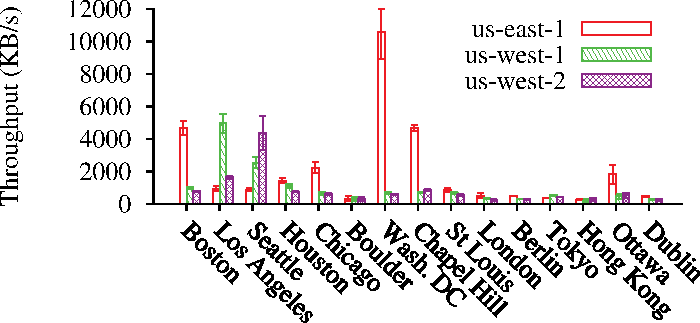
\includegraphics[width=0.55\textwidth]{./figures/cloudmeasure/imag_sec5/region_bandwidth.pdf}
\caption{Average throughput between representative clients and EC2 regions in the US.}
\label{fig:region_bandwidth}
\end{figure}

\begin{figure}[t]
\centering
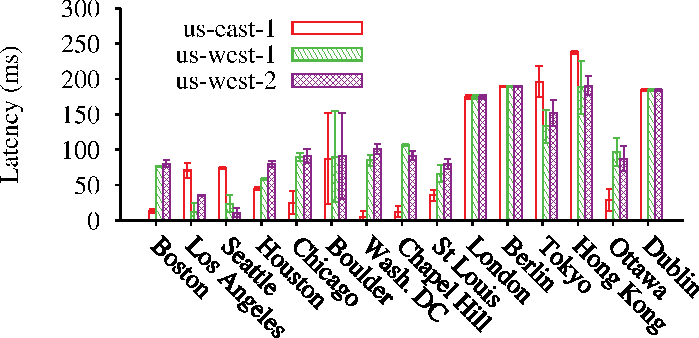
\includegraphics[width=0.55\textwidth]{./figures/cloudmeasure/imag_sec5/region_latency.pdf}
\caption{Average latency between representative clients and EC2 regions in the US.}
\label{fig:region_latency}
\end{figure}


\tightparagraph{Performance across different regions.}
Figures~\ref{fig:region_bandwidth} and \ref{fig:region_latency} show the
latency and throughput measurements for 15 representative PlanetLab
locations and for the three US EC2 regions. The PlanetLab nodes are spread
across the US and other parts of the world. 
%\tnote{How were these selected? Why is
%it different across the different charts?}
We make a few key observations: ({\em i}) Single-region deployments must
carefully choose a region. For example, the two US west
regions do not offer equivalent ``across-the-board'' performance, with
ec2.us-west-1 offering better average latency and throughput (130 ms
and 1143 KB/s) than ec2.us-west-2 (145 ms and 895 KB/s)
(averaged across all client locations). ({\em ii}) The charts show that the
region chosen to serve content to a given client can have a
significant performance impact. For example, for the client in
Seattle, using the ec2.us-west-2 region can reduce latency by close to
a factor of 6 and improve throughput by close to a factor of 5
compared to using ec2.us-east-1. ({\em iii}) We also note that the way a
region is chosen may depend on the client's location: always choosing
ec2.us-west-1 for the Seattle client is a good idea, but for the
client in Boulder, the best choice of region may change
dynamically.

\iffalse
\begin{figure}[!t]
\centering
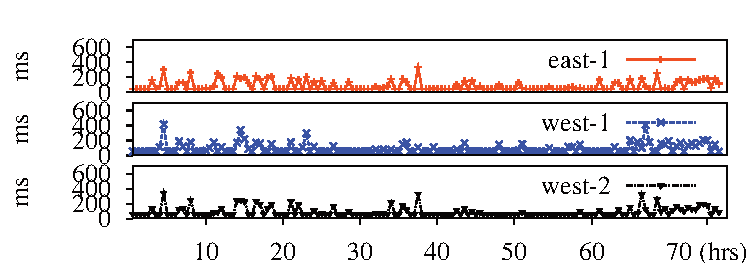
\includegraphics[width=0.55\textwidth]{./figures/cloudmeasure/imag_sec5/sec5_latency_colorado.pdf}
\caption{Latencies between Boulder site and three EC2 US regions. The
  best performing region changes over time.}
\label{fig:boulder_latency}
\end{figure}
\fi

We now examine the relative benefits of, and choices underlying,
multi-region deployments in more detail. We start by deriving an upper
bound on the performance from a $k$-region deployment of a service. To
do this, we determine the best $k$ regions out of the 8, for $1 \le k
\le 8$.  Using our measurement data we determine the overall
performance that the clients would have achieved given a routing
algorithm that picked the optimal region from the $k$ for each client
and at each point in time. More specifically, for each value of $k$
we: ({\em i}) enumerate all size-$k$ subsets of regions; ({\em ii}) for each
size-$k$ subset compute the average performance across all clients
assuming each client uses the lowest latency or highest throughput
region of the $k$ at each time round (15 min); 
and ({\em iii}) choose from these the size-$k$ subset with lowest latency or
highest throughput.
\figref{fig:multi_region_latency_bandwidth} shows the results. We find that while average performance can be increased a
significant amount by adding more regions to one's deployment, there
is evidence of diminishing returns after $k=3$. In particular, latency
decreases by 33\% when $k=3$ compared to $k=1$, but only decreases by
39\% when $k=4$.

We now examine what constitutes the best $k$ regions to use. The
choice of best regions, by throughput, is as follows: \awseast
($k=1$); \awseast ,\awseuro($k=2$); \awseast, \awseuro, \awscali
($k=3$); and \awseast, \awseuro, \awscali, \awssing ($k=4$).
%\tnote{This statement is a bit ambiguous. 
%Do we mean that it provided the highest on average across all regions?
%We should then answer the natural question of whether 
%people are using US East because it's so good (maybe push to a discussion 
%section later though).}  
The choice of best regions, by latency, is: \awseast
($k=1$); \awseast,\awstokyo ($k=2$); \awseast, \awstokyo, \awscali
($k=3$); and \awseast, \awstokyo, \awscali, \awssing ($k=4$).



\tightparagraph{Performance across different zones.} We also investigated the
difference in performance should one use different zones in the
same region. % \figref{fig:zone_bandwidth} and \figref{fig:zone_latency}
% give the latency and throughput for the three \awseast zones as seen
% from clients in 15 representative cities.
We found that the zone has
little impact on latency, with almost equivalent average RTTs for all
clients across the two days (results omitted for brevity). For throughput, the variation appears to
be somewhat higher, but not as significant as that seen across
regions. % For some periods in time, better throughput is seen to one
% zone than the other.
We believe such variation is due to local
effects, such as contention on shared instances or network
switches. % \tnote{The implications are stronger in that the averages
%   over time are also different, at least for the Boston
%   example. Should we say so or is it too slight to be significant?}
% \aditya{seems small to me..} 
This is suggested as well by other
recent measurements of EC2 performance
variability~\cite{farley:gaming:socc:2012}.  Moreover, in the next
section we show that the Internet path variability between zones is
low as well.

\tightparagraph{Summary and Implications} We find that using multiple
regions can improve latency and throughput significantly. However,
leveraging multiple regions may not be easy: while a given region
always offers best performance for some clients, the choice of region
for other clients will have to adapt in an online dynamic
fashion. This could be achieved via global request scheduling (effective,
but complex) or requesting from multiple regions in parallel (simple,
but increases server load).

While a multiple region deployment helps improve web service 
performance and protects against major cloud failures, cloud tenants must
also consider other factors in making their decision of how many and which
regions to use. First, cloud providers charge for inter-region network
traffic, potentially causing tenants to incur additional charges when
switching to a multi-region deployment. Second, the design of particular
cloud features may restrict how a tenant's data can be shared across regions:
e.g., objects stored in Amazon's Simple Storage Service (S3) can only be
stored in one region at a time and Amazon Machine Images (AMIs) cannot be
shared between regions. Lastly, deployments that rely on fewer features may be
less susceptible to failures---e.g., deployments which only use VMs, and not
other services like Amazon Elastic Block Storage or Amazon ELB, have not been
affected by some major 
outages~\cite{AWSoutageOct2012,AWSoutageDec2012}---reducing the need for resiliency through the use of multiple regions.


\begin{figure}[tb]
\centering
	\begin{subfigure}[b]{0.4\textwidth}
                \centering
                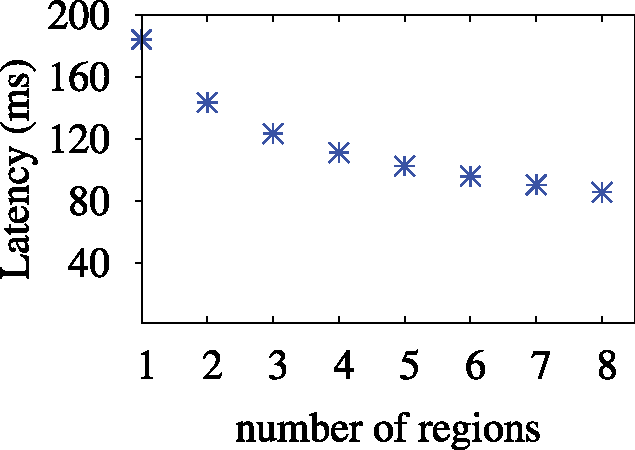
\includegraphics[width=\textwidth]{./figures/cloudmeasure/imag_sec5/sec5_region_latency_impr_fix.pdf}
		\caption{Latency}
	\end{subfigure}
	\begin{subfigure}[b]{0.4\textwidth}
                \centering
                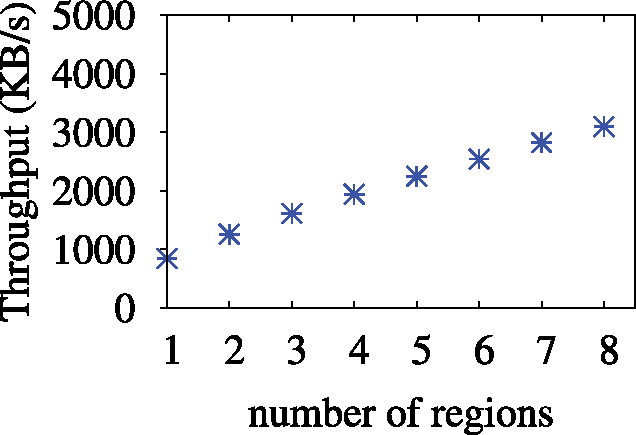
\includegraphics[width=\textwidth]{./figures/cloudmeasure/imag_sec5/sec5_region_speed_impr_fix.pdf}
		\caption{Throughput}
	\end{subfigure}
	\caption{Average latency/throughput across all clients using an optimal $k$-region
	deployment.}
	\label{fig:multi_region_latency_bandwidth}
\end{figure}

\subsubsection{ISP Diversity}

We now investigate tolerance to wide-area faults. Having in previous sections
already established the reliance of many cloud-using services on one zone or region,
we now focus on diversity in the immediate downstream ISPs at each EC2 zone. Greater
diversity, and an even spread of routes across downstream ISPs,
generally indicates greater tolerance to failures in Internet routing.

\begin{table}[t]
\centering\small
\begin{tabular}{|c||c|c|c|} \hline
\bf Region & \bf AZ1 &  \bf AZ2 &  \bf AZ3  \\ \hline
ec2.us-east-1 &  36 & 36 & 34\\ \hline
ec2.us-west-1 & 18 & 19 & n/a\\ \hline
ec2.us-west-2 &  19 & 19 & 19\\ \hline
ec2.eu-west-1&  10 & 11 & 13\\ \hline
ec2.ap-northeast-1 & 9 & n/a & 9\\ \hline
ec2.ap-southeast-1 &  11 & 12 & n/a\\ \hline
ec2.ap-southeast-2&    4 & 4 & n/a\\ \hline
ec2.sa-east-1 &  4 & 4& n/a\\ \hline
\end{tabular}

\caption{Number of downstream ISPs for each EC2 region and zone.}
\label{as_number}
\end{table}

To do this study, we set up three m1.medium instances in each of the
available EC2 availability zones.  Then we ran \emph{traceroute}
50 times from each of these instances to each of 200 geographically
diverse PlanetLab nodes (\figref{fig:nodes_deploy}).  Finally, we used
the UNIX `whois' utility to
determine the autonomous system (AS) number associated with the first non-EC2
hop, and we count that AS as an immediate downstream ISP for the zone hosting 
the instance. The discovered ASs constitute a lower bound for the true number of ASs.
\tabref{as_number} gives the number of distinct
ASs seen for each zone and region.
We note that:
({\em i}) different zones in a region have (almost) the same number of
  downstream ISPs; and
({\em ii}) the extent of diversity varies across regions, with some
  connected to more than 30 downstream ISPs and others
  connected to just 4. Except for South America and Asia Pacific
  Sydney, other regions are well-multihomed.


We also studied the spread of routes across downstream ISPs (not
shown). We found it to be rather uneven: even when using
well-connected regions -- e.g., \awscali and \awseuro -- we found that
up to 31\% (\awscali) and 33\% (\awseuro) of routes use the same
downstream ISP.

\tightparagraph{Summary and Implications} Although individual regions are
multihomed, the uneven spread of routes implies that local failures in
downstream ISPs can cause availability problems for large fractions of
clients of cloud-using web services. This could be overcome by using
multiple regions at once, or by leveraging dynamic route control
solutions~\cite{akella2004multihoming}.

%%%%%%%%%%%%%%%%%%%%%%%%%%%%%%%%%%%%%%%%%%%%%%%%%%%%%%%%%%%%%%%%%%%%%%%%%%%%%%%%

